\documentclass[11pt,openany]{article}
\usepackage[dutch]{babel}
\usepackage{amsmath}
\usepackage{amssymb}
\usepackage{graphicx}
\usepackage{enumitem}
\usepackage[center]{caption}
\usepackage{a4wide}
\setcounter{tocdepth}{1}
\setlength{\parindent}{0pt}
\usepackage{multirow}
\usepackage{fancyhdr}
\usepackage{blindtext}
\usepackage{pdfpages}


\begin{document}

\includepdf[pages={1}]{voorblad.pdf}

	
	\tableofcontents
	\newpage
	
\section{Introductie}

\subsection{Wat is Solvas Fleet?}
Solvas Fleet is een web based applicatie die instaat voor het beheren van klant- en polisgegevens van een voertuigvloot. Met Solvas Fleet is het mogelijk om ten alle tijde deze gegevens te kunnen beheren zonder daarbij te moeten wachten op informatie of zich te verplaatsen.  Hierbij zal Solvas Fleet steeds een duidelijk overzicht van de gegevens voorzien die u nodig heeft en dit in een beveiligde omgeving.\\

Deze gebruikershandleing heeft als doel de gebruiker een zo aangenaam mogelijke ervaring met Solvas Fleet te garanderen en biedt voldoende informatie om een gebruiker zonder enige voorkennis volledig te kunnen assisteren bij het proces.
\subsection{Wat is mogelijk met Solvas Fleet?}
Zoals reeds vermeld, wordt Solvas Fleet gebruikt om klant- en polisgegevens van vloten te beheren. De applicatie laat hierbij toe deze gegevens te raadplegen, of met de nodige rechten, ook te kunnen inbrengen,wijzigen of verwijderen uit het systeem. In deze versie van Solvas Fleet wordt onderstaande functionaliteit ondersteund:


\begin{itemize}[noitemsep]
	\item \textbf{Gebruiker}: aanmaken/wijzigen/verwijderen/lijst weergeven
	\item \textbf{Klant}: aanmaken/wijzigen/verwijderen/lijst weergeven
	\item \textbf{Vloot}: aanmaken/wijzigen/verwijderen/lijst weergeven
	\item \textbf{Voertuig}: aanmaken/wijzigen/verwijderen/lijst weergeven
	\item Lijst van alle vloten van een klant weergeven
	\item Lijst van alle voertuigen van een vloot weergeven
	\item Lijst van alle voertuigen van een bepaald type weergeven
\end{itemize}

\newpage
\section{Gebruiker}
\subsection{Gebruiker aanmaken}
Om een gebruiker aan te maken, volgt u onderstaande stappen:
\begin{enumerate}
	\item Start de Solvas Fleet applicatie. U ziet het startscherm weergegeven in Figuur 1.
	\item In de zijbalk kiest u voor 'Gebruikers'. U ziet nu een lijst van alle gebruikers zoals weergegeven in Figuur 2.
	\item Om een gebruiker toe te voegen, klikt u op het plus icoon onderaan de pagina. Dit icoon is op Figuur 2 aangeduid in het rood.
	\item U krijgt nu een formulier te zien zoals	 in Figuur 3 met als titel 'Gebruiker aanmaken'.
	\item Vul het formulier op een correcte manier in en bevestig het aanmaken van een gebruiker door het groene icoontje aan te klikken (stap 6) of annuleer het proces via het rode icoontje (stap 8) .
	\item Indien u het aanmaken van een gebruiker bevestigt, komt u terecht op de informatiepagina van de gebruiker zoals weergegeven in Figuur 4. 
	\item Indien u wenst terug te keren  naar de lijst van gebruikers, klikt u de knop 'Terug' aan.
	\item Indien u het aanmaken van een gebruiker annuleert, komt u opnieuw terecht bij de lijst van gebruikers 
\end{enumerate}
	
	\begin{figure}
		\centering
		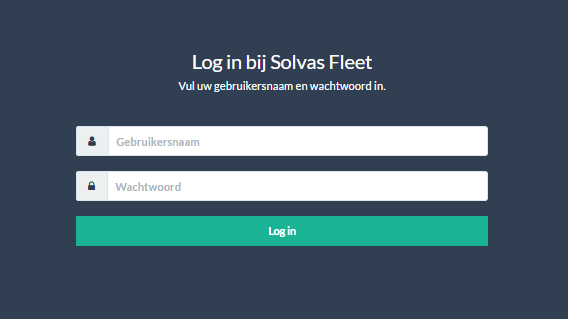
\includegraphics[width=0.9\textwidth]{fig1.png}
		\caption{Startscherm Solvas Fleet}
	\end{figure}

\begin{figure}
	\centering
	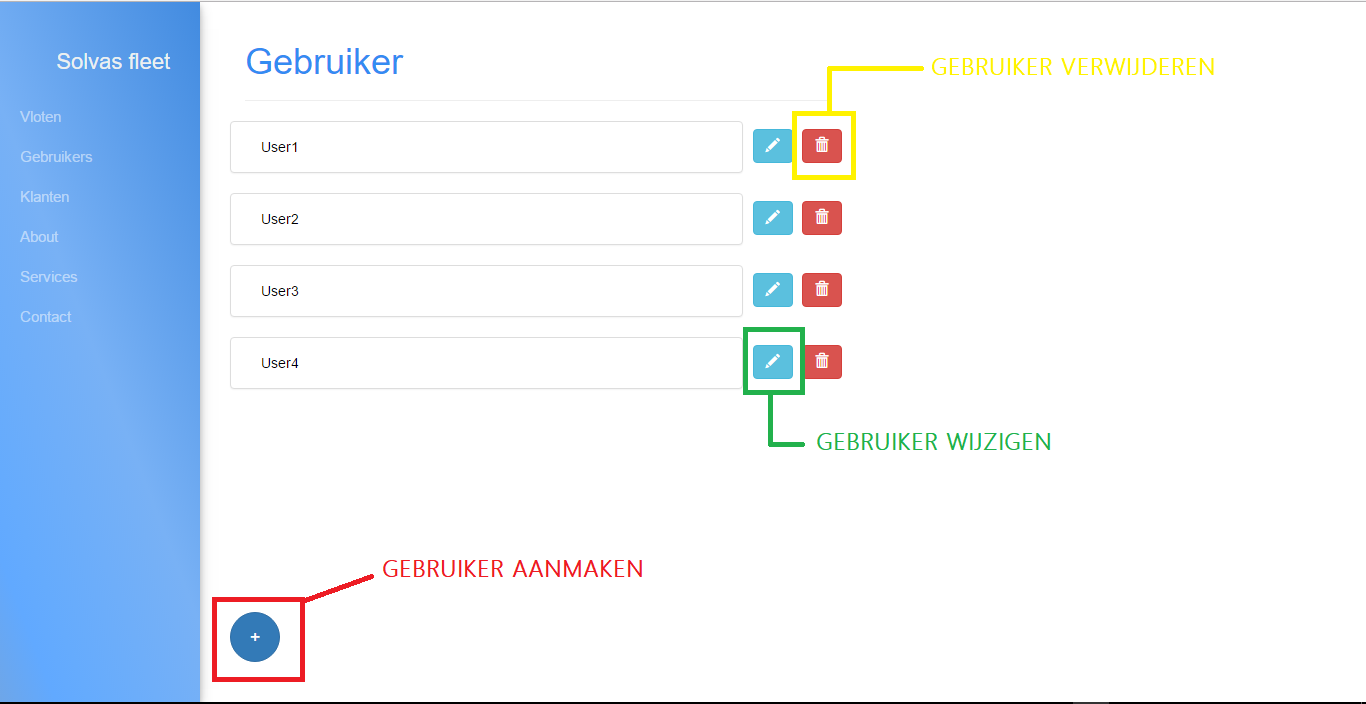
\includegraphics[width=0.9\textwidth]{fig2.png}
	\caption{Lijst van gebruikers}
\end{figure}
	
\begin{figure}
	\centering
	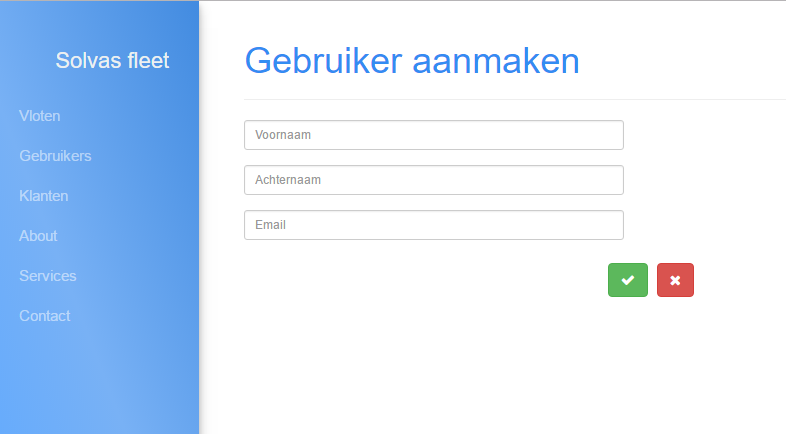
\includegraphics[width=0.9\textwidth]{fig3.png}
	\caption{Formulier gebruiker}
\end{figure}

\newpage
\subsection{Gebruiker wijzigen}
Om een gebruiker te wijzigen, volgt u onderstaande stappen:
\begin{enumerate}
	\item Start de Solvas Fleet applicatie. U ziet het startscherm weergegeven in Figuur 1.
	\item In de zijbalk kiest u voor 'Gebruikers'. U ziet nu een lijst van alle gebruikers zoals weergegeven in Figuur 2.
	\item Om een gebruiker te wijzigen, klikt u het lichtblauwe penseel icoon aan. Dit icoon is op Figuur 2 aangeduid in het groen.
	\item U krijgt nu een formulier te zien zoals in Figuur 3 met als titel 'Gebruiker aanpassen'.
	\item Vul het formulier op een correcte manier in en bevestig het wijzigen van een gebruiker door het groene icoontje aan te klikken (stap 6) of annuleer het proces via het rode icoontje (stap 8) .
	\item Indien u het wijzigen van een gebruiker bevestigt, komt u terecht op de informatiepagina van de gebruiker zoals weergegeven in Figuur 4. 
	\item Indien u wenst terug te keren naar de lijst van gebruikers, klikt u de knop 'Terug' aan.
	\item Indien u het wijzigen van een gebruiker annuleert, komt u opnieuw terecht bij de lijst van gebruikers 
\end{enumerate}

\subsection{Gebruiker verwijderen}
Om een gebruiker te verwijderen, volgt u onderstaande stappen:
\begin{enumerate}
	\item Start de Solvas Fleet applicatie. U ziet het startscherm weergegeven in Figuur 1.
	\item In de zijbalk kiest u voor 'Gebruikers'. U ziet nu een lijst van alle gebruikers zoals weergegeven in Figuur 2.
	\item Om een gebruiker te verwijderen, klikt u op het rode vuilbak icoon. Dit icoon is op Figuur 2 aangeduid in het geel.
	\item De applicatie vraagt om een extra bevestiging. Indien u wilt doorgaan met het verwijderen, kiest u voor 'ok'. In het andere geval kiest u voor 'annuleren'.
	\item Het systeem verwijdert de door u gekozen gebruiker en u bevindt zich opnieuw naar de lijst van gebruikers (Figuur 2).
\end{enumerate}
\newpage
\subsection{Lijst van alle gebruikers weergeven}
Om een lijst van gebruikers te verkrijgen, volgt u onderstaande stappen:
\begin{enumerate}
		\item Start de Solvas Fleet applicatie. U ziet het startscherm weergegeven in Figuur 1.
		\item In de zijbalk kiest u voor 'Gebruikers'. U ziet nu een lijst van alle gebruikers zoals weergegeven in Figuur 2.
		\item Indien u meer informatie wenst over een gebruiker, klikt u op de desgewenste gebruiker. 
		\item U ziet nu informatie over de gekozen gebruiker zoals weergegeven in Figuur 4. 
		\item Indien u wenst terug te keren naar de lijst van gebruikers, klikt u de knop 'Terug' aan.
\end{enumerate}

\begin{figure}
	\centering
	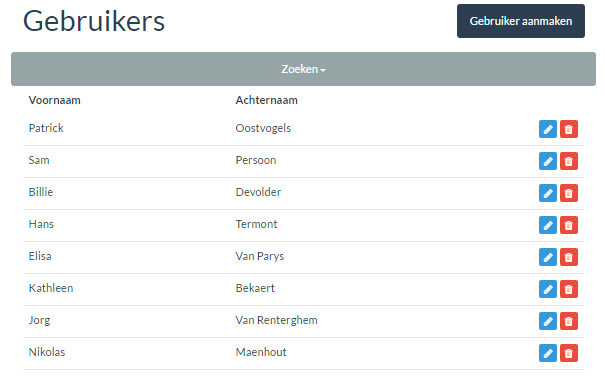
\includegraphics[width=0.9\textwidth]{fig4.png}
	\caption{Informatie over gebruiker}
\end{figure}


\newpage

\section{Klant}
\subsection{Klant aanmaken}
Om een klant aan te maken, volgt u onderstaande stappen:
\begin{enumerate}
	\item Start de Solvas Fleet applicatie. U ziet het startscherm weergegeven in Figuur 1.
	\item In de zijbalk kiest u voor 'Klanten'. U ziet nu een lijst van alle klanten zoals weergegeven in Figuur 5.
	\item Om een klant toe te voegen, klikt u op het plus icoon onderaan de pagina. Dit icoon is op Figuur 5 aangeduid in het rood.
	\item U krijgt nu een formulier te zien zoals in Figuur 6 met als titel 'Klant aanmaken'.
	\item Vul het formulier op een correcte manier in en bevestig het aanmaken van een klant door het groene icoontje aan te klikken (stap 6) of annuleer het proces via het rode icoontje (stap 8) .
	\item Indien u het aanmaken van een klant bevestigt, komt u terecht op de informatiepagina van de klant zoals weergegeven in Figuur 7. 
	\item Indien u wenst terug te keren  naar de lijst van klanten, klikt u de knop 'Terug' aan.
	\item Indien u het aanmaken van een klant annuleert, komt u opnieuw terecht bij de lijst van klanten .
\end{enumerate}
\begin{figure}
	\centering
	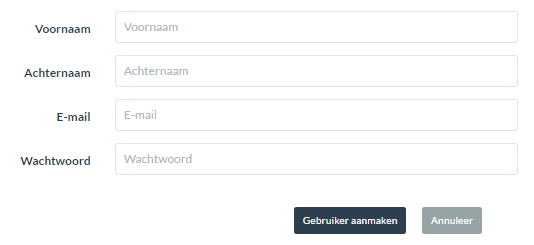
\includegraphics[width=0.9\textwidth]{fig5.png}
	\caption{Lijst van klanten}
\end{figure}

\begin{figure}
	\centering
	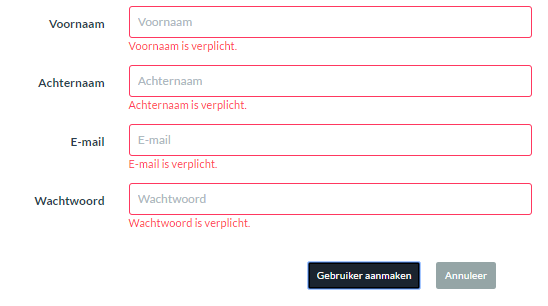
\includegraphics[width=0.9\textwidth]{fig6.png}
	\caption{Formulier klanten}
\end{figure}
\newpage
\subsection{Klant wijzigen}
Om een klant te wijzigen, volgt u onderstaande stappen:
\begin{enumerate}
	\item Start de Solvas Fleet applicatie. U ziet het startscherm weergegeven in Figuur 1.
	\item In de zijbalk kiest u voor 'Klanten'. U ziet nu een lijst van alle gebruikers zoals weergegeven in Figuur 5.
	\item Om een klant te wijzigen, klikt u op het lichtblauwe penseel icoon. Dit icoon is op Figuur 5 aangeduid in het groen.
	\item U krijgt nu een formulier te zien zoals in Figuur 6 met als titel 'Klant aanpassen'.
	\item Vul het formulier op een correcte manier in en bevestig het wijzigen van een klant door het groene icoontje aan te klikken (stap 6) of annuleer het proces via het rode icoontje (stap 8) .
	\item Indien u het wijzigen van een klant bevestigt, komt u terecht op de informatiepagina van de klant zoals weergegeven in Figuur 7. 
	\item Indien u wenst terug te keren  naar de lijst van klanten, klikt u de knop 'Terug' aan.
	\item Indien u het wijzigen van een klant annuleert, komt u opnieuw terecht bij de lijst van klanten .
\end{enumerate}

\subsection{Klant verwijderen}
Om een klant te verwijderen, volgt u onderstaande stappen:
\begin{enumerate}
	\item Start de Solvas Fleet applicatie. U ziet het startscherm weergegeven in Figuur 1.
	\item In de zijbalk, kiest u voor 'Klant'. U ziet nu een lijst van alle klanten zoals weergegeven in Figuur 2.
	\item Om een klant te verwijderen, klikt u op het rode vuilbak icoon. Dit icoon is op Figuur 5 aangeduid in het geel.
	\item De applicatie vraagt om een extra bevestiging. Indien u wilt doorgaan met het verwijderen, kiest u voor 'ok'. In het andere geval kiest u voor 'annuleren'.
	\item Het systeem verwijdert de door u gekozen klant en u bevindt zicht opnieuw naar de lijst van klanten (Figuur 5).
\end{enumerate}

\subsection{Lijst van alle klanten weergeven}
Om een lijst van klanten te verkrijgen, volgt u onderstaande stappen:
\begin{enumerate}
	\item Start de Solvas Fleet applicatie. U ziet het startscherm weergegeven in Figuur 1.
	\item In de zijbalk kiest u voor 'Klanten'. U ziet nu een lijst van alle klanten zoals weergegeven in Figuur 5.
	\item Indien u meer informatie wenst over een klant, klikt u op de desgewenste klant. 
	\item U ziet nu informatie over de gekozen klant zoals weergegeven in Figuur 7. 
	\item Indien u wenst terug te keren naar de lijst van klanten, klikt u de knop 'Terug' aan.
\end{enumerate}

\begin{figure}
	\centering
	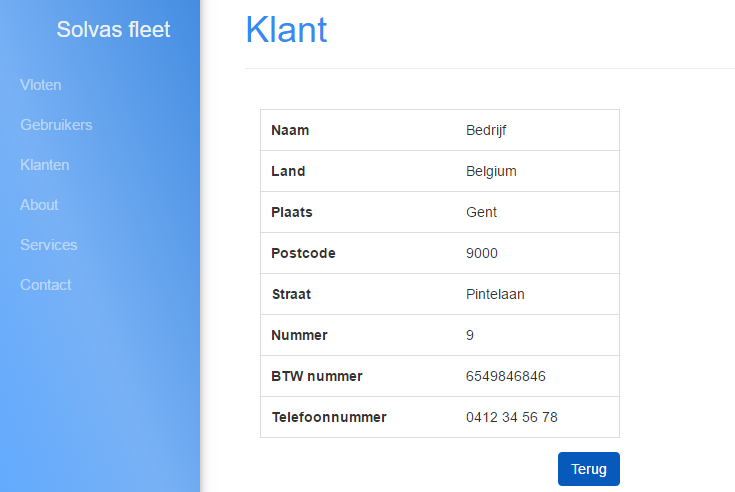
\includegraphics[width=0.9\textwidth]{fig7.png}
	\caption{Informatie over klant}
\end{figure}
\newpage
\section{Vloot}
\subsection{Vloot van een klant aanmaken}
Om een vloot voor een klant aan te maken, volgt u onderstaande stappen:
\begin{enumerate}
	\item Start de Solvas Fleet applicatie. U ziet het startscherm weergegeven in Figuur 1.
	\item In de zijbalk kiest u voor 'Vloten'. U ziet nu een lijst van alle vloten van de klant zoals weergegeven in Figuur 8.
	\item Om een vloot toe te voegen, klikt u op het plus icoon onderaan de pagina. Dit icoon is op Figuur 8 aangeduid in het rood.
	\item U krijgt nu een formulier te zien zoals in Figuur 9 met als titel 'Nieuwe vloot'.
	\item Vul het formulier op een correcte manier in en bevestig het aanmaken van een vloot door het groene icoontje aan te klikken (stap 6) of annuleer het proces via het rode icoontje (stap 8) .
	\item Indien u het aanmaken van een vloot bevestigt, komt u terecht op de informatiepagina van de vloot zoals weergegeven in Figuur 10. 
	\item Indien u wenst terug te keren  naar de lijst van vloten, klikt u de knop 'Terug' aan.
	\item Indien u het aanmaken van een vloot annuleert, komt u opnieuw terecht bij de lijst van vloten 
\end{enumerate}

\begin{figure}
	\centering
	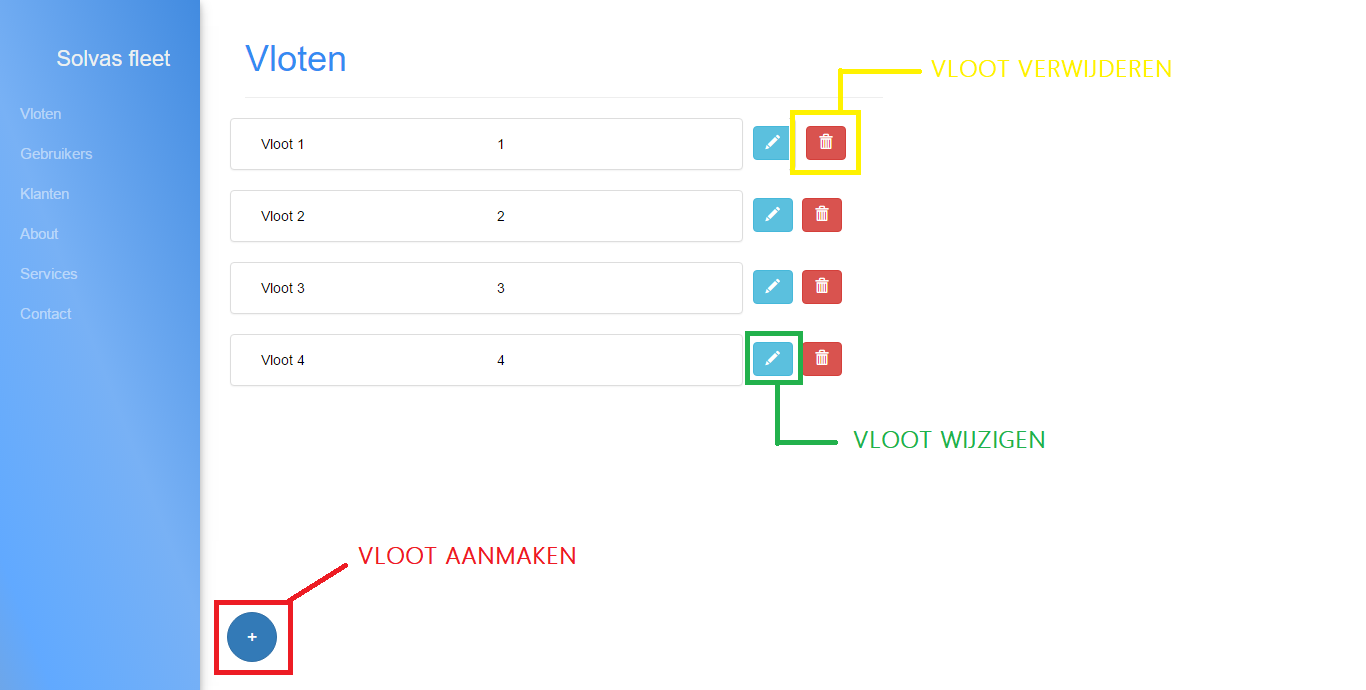
\includegraphics[width=0.9\textwidth]{fig8_2.png}
	\caption{Lijst van vloten}
\end{figure}

\begin{figure}
	\centering
	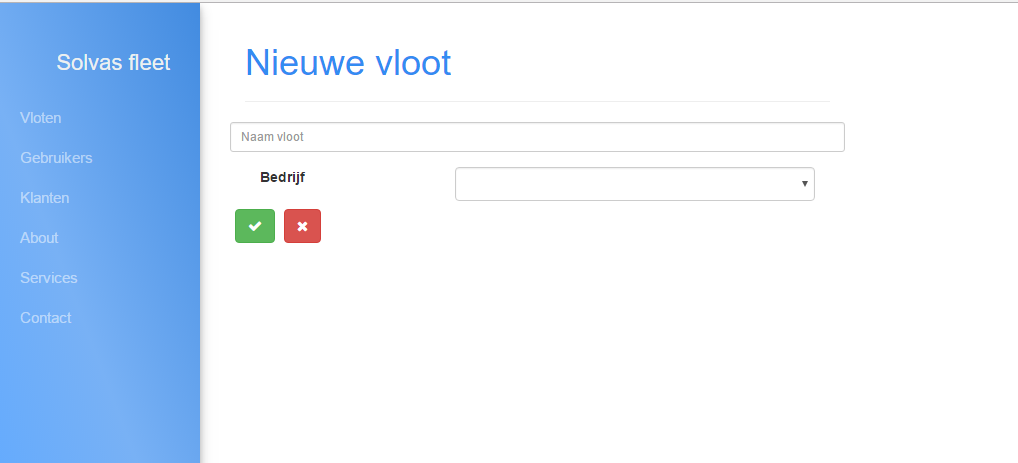
\includegraphics[width=0.9\textwidth]{fig9.png}
	\caption{Formulier vloot}
\end{figure}
\newpage

\subsection{Vloot wijzigen}
Om een vloot te wijzigen, volgt u onderstaande stappen:
\begin{enumerate}
	\item Start de Solvas Fleet applicatie. U ziet het startscherm weergegeven in Figuur 1.
	\item In de zijbalk kiest u voor 'Vloten'. U ziet nu een lijst van alle vloten van de klant zoals weergegeven in Figuur 8.
	\item Om een vloot te wijzigen, klikt u op het lichtblauwe penseel icoon. Dit is op Figuur 8 aangeduid in het groen
	\item U krijgt nu een formulier te zien zoals in Figuur 9 met als titel 'Wijzig vloot'.
	\item Vul het formulier op een correcte manier in en bevestig het wijzigen van een vloot door het groene icoontje aan te klikken (stap 6) of annuleer het proces via het rode icoontje (stap 8) .
	\item Indien u het wijzigen van een vloot bevestigt, komt u terecht op de informatiepagina van de vloot zoals weergegeven in Figuur 10. 
	\item Indien u wenst terug te keren  naar de lijst van vloten, klikt u de knop 'Terug' aan.
	\item Indien u het wijzigen van een vloot annuleert, komt u opnieuw terecht bij de lijst van vloten 
\end{enumerate}

\subsection{Vloot verwijderen}
Om een Vloot te verwijderen, volgt u onderstaande stappen:
\begin{enumerate}
	\item Start de Solvas Fleet applicatie. U ziet het startscherm weergegeven in Figuur 1.
	\item In de zijbalk kiest u voor 'Vloten'. U ziet nu een lijst van alle vloten zoals weergegeven in Figuur 8.
	\item Om een vloot te verwijderen, klikt u op het rode vuilbak icoon. Dit icoon is op Figuur 8 aangeduid in het geel.
	\item Het systeem verwijdert de door u gekozen vloot en u bevindt zicht opnieuw naar de lijst van vloten (Figuur 5).
\end{enumerate}

\subsection{Lijst van alle vloten van een klant weergeven}
Om een lijst van vloten te verkrijgen, volgt u onderstaande stappen:
\begin{enumerate}
	\item Start de Solvas Fleet applicatie. U ziet het startscherm weergegeven in Figuur 1.
	\item In de zijbalk kiest u voor 'Vloten'. U ziet nu een lijst van alle vloten van een klant zoals weergegeven in Figuur 8.
	\item Indien u meer informatie wenst over een vloot, klikt u op de desgewenste vloot. 
	\item U ziet nu informatie over de gekozen vloot (afhankelijk van type voertuigen)
	ongeveer zoals weergegeven in Figuur 10. Voor de verdere functionaliteit van deze pagina zie sectie 5 over Voertuigen. 
	\item Indien u wenst terug te keren naar de lijst van vloten, kiest u de pijl naar links  linksbovenaan in de browser om terug te keren naar de vorige pagina.
\end{enumerate}

\begin{figure}
	\centering
	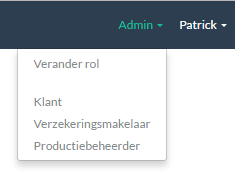
\includegraphics[width=0.9\textwidth]{fig10.png}
	\caption{Informatie over vloot}
\end{figure}

\newpage
\section{Voertuig}
\subsection{Voertuig aanmaken}
Om een voertuig voor een vloot aan te maken, volgt u onderstaande stappen:
\begin{enumerate}
	\item Start de Solvas Fleet applicatie. U ziet het startscherm weergegeven in Figuur 1.
	\item In de zijbalk kiest u voor 'Vloten'. U ziet nu een lijst van alle vloten van de klant zoals weergegeven in Figuur 8.
	\item Om een voertuig toe te voegen, klikt u op de gewenste vloot waarvoor u een nieuw voertuig wilt toevoegen. 
	\item U krijgt nu een pagina te zien met de informatie (subvloten en voertuigen) van de gekozen vloot
	ongeveer zoals weergegeven in Figuur 10. 
	\item Om een voertuig toe te voegen klikt u de knop 'Nieuw Voertuig' aan.
	\item U krijgt nu een formulier te zien zoals in Figuur 11 met als titel 'Nieuw voertuig'.
	\item Vul het formulier op een correcte manier in en bevestig het aanmaken van een voertuig door het groene icoontje aan te klikken (stap 6) of annuleer het proces via het rode icoontje (stap 8) .
	\item Indien u het aanmaken van een voertuig bevestigt, komt u terecht op de informatiepagina van het voertuig zoals weergegeven in Figuur 10. 
	\item Indien u wenst terug te keren  naar informatiepagina van de vloot, klikt u de knop 'Terug' aan.
	\item Indien u het aanmaken van een voertuig annuleert, komt u opnieuw terecht bij de informatiepagina over de vloot.
\end{enumerate}


\begin{figure}
	\centering
	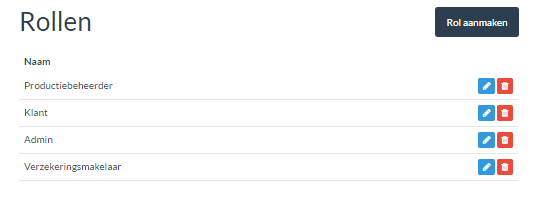
\includegraphics[width=0.9\textwidth]{fig11.png}
	\caption{Formulier voertuig}
\end{figure}

\subsection{Voertuig wijzigen}
Om een voertuig voor een vloot te wijzigen, volgt u onderstaande stappen:
\begin{enumerate}
	\item Start de Solvas Fleet applicatie. U ziet het startscherm weergegeven in Figuur 1.
	\item In de zijbalk kiest u voor 'Vloten'. U ziet nu een lijst van alle vloten van de klant zoals weergegeven in Figuur 8.
	\item Om een voertuig te wijzigen, klikt u op de gewenste vloot waarvoor u een voertuig wilt wijzigen. 
	\item U krijgt nu een pagina te zien met de informatie (subvloten en voertuigen) van de gekozen vloot
	ongeveer zoals weergegeven in Figuur 10. 
	\item Om een voertuig te wijzigen klikt u op het lichtblauwe penseel icoon. Dit is op Figuur 10 aangeduid in het groen.
	\item U krijgt nu een formulier te zien zoals in Figuur 11 met als titel 'Wijzig voertuig'.
	\item Vul het formulier op een correcte manier in en bevestig het wijzigen van een voertuig door het groene icoontje aan te klikken (stap 6) of annuleer het proces via het rode icoontje (stap 8) .
	\item Indien u het wijzigen van een voertuig bevestigt, komt u terecht op de informatiepagina van het voertuig zoals weergegeven in Figuur 10. 
	\item Indien u wenst terug te keren  naar de lijst van voertuigen, klikt u de knop 'Terug' aan. U komt terecht op de informatiepagina van de vloot indien het voertuig tot deze vloot behoort. In het ander geval komt u opnieuw terecht bij de lijst van vloten.
	\item Indien u het wijzigen van een vloot annuleert, komt u opnieuw terecht bij de lijst van vloten 
\end{enumerate}

\subsection{Voertuig verwijderen}
Om een voertuig voor een vloot te verwijderen, volgt u onderstaande stappen:
\begin{enumerate}
	\item Start de Solvas Fleet applicatie. U ziet het startscherm weergegeven in Figuur 1.
	\item In de zijbalk kiest u voor 'Vloten'. U ziet nu een lijst van alle vloten van de klant zoals weergegeven in Figuur 8.
	\item Om een voertuig te verwijderen, klikt u op de gewenste vloot waarvoor u een voertuig wilt verwijderen. 
	\item U krijgt nu een pagina te zien met de informatie (subvloten en voertuigen) van de gekozen vloot
	ongeveer zoals weergegeven in Figuur 10. 
	\item Om een voertuig te wijzigen klikt u op het rode vuilbak icoon. Dit is op Figuur 10 aangeduid in het geel.
	\item Het systeem verwijdert het door u gekozen voertuig en u bevindt zicht opnieuw naar de informatiepagina van uw vloot.
\end{enumerate}


\subsection{Lijst van alle voertuigen (van een bepaald type) van een vloot weergeven}
\begin{enumerate}
	\item Start de Solvas Fleet applicatie. U ziet het startscherm weergegeven in Figuur 1.
	\item In de zijbalk kiest u voor 'Vloten'. U ziet nu een lijst van alle vloten van de klant zoals weergegeven in Figuur 8.
	\item Om een lijst van voertuigen te verkrijgen, klikt u op de gewenste vloot.
	\item U krijgt nu een pagina te zien met de informatie (subvloten en voertuigen) van de gekozen vloot
	ongeveer zoals weergegeven in Figuur 10. Hier ziet u alle voertuigen die bij deze vloot horen onderverdeeld in subvloten per voertuigtype.
\end{enumerate}





\end{document}
